%Ceci est le fichier à compiler pour avoir le pdf
%le document se trouve dans document.tex
%les fichiers qui commencent par "system_" sont des trucs "systèmes"... bref les trucs moches de latex dont tout le monde s'en fout
%les fichiers qui commencent par "document_" sont les fichiers "jolis". Pas de trucs GeEkS dedans svp !!



% *** document class ***
\documentclass[a4paper,8pt]{article}
%
% Toutes les options de documentclass sont transmises à toutes les
% commandes «\usepackage».
%

\usepackage[utf8]{inputenc}     % UTF 8
%\usepackage{xspace} %space after a command
%\usepackage{eurosym} %for the symbol euro



% pour faire des calculs dans les commandes latex
\usepackage{calc}
\usepackage[T1]{fontenc}

% explicite
\usepackage{url}

% *** color ***
\usepackage{color}

% Tikz a besoin d'au moins ces versions
\def\xkeyvalversion{1.8}
\def\xcolorversion{2.00}

\usepackage{pgf}
\usepackage{pgfcore}
%\usepackage{pgfbaseimage}
%\usepackage{pgfbaselayers}
%\usepackage{pgfbasepatterns}
%\usepackage{pgfbaseplot}
\usepgfmodule{plot}
%\usepackage{pgfbaseshapes}
\usepgfmodule{shapes}
%\usepackage{pgfbasesnakes}
\usepgfmodule{decorations}
\usepackage{tikz}
% chargement des composants
%\usetikzlibrary{arrows,patterns,plotmarks,shapes,snakes,er,3d,automata,backgrounds,topaths,trees,petri,mindmap}
\usetikzlibrary{arrows,patterns,plotmarks,er,3d,automata,backgrounds,topaths,trees,petri,mindmap}
% d'autres librairies possibles : matrix, calendar, folding


\usepackage{graphicx}

% *** array ***
% étend les options des environnements «array» et «tabular»
\usepackage{array}



% packages matheux
\usepackage{amsmath}
\usepackage{amssymb}  % \mathbb
\DeclareMathAlphabet{\mathpzc}{OT1}{pzc}{m}{it} % \mathpzc
%\usepackage{dsfont}   % \mathds
\usepackage{mathrsfs} % \mathscr



\usepackage{fancyvrb}
%\usepackage{verbdef}


% *** draftcopy ***
% imprime «brouillon» en fond de page
%\usepackage{draftcopy}



%\usepackage{hyperref}
\usepackage[bookmarks={true},bookmarksopen={true}]{hyperref}
%\usepackage[colorlinks=true,linkcolor=blue,urlcolor=blue]{hyperref}
%pour faire un pdf avec une table des matières
%\hypersetup{colorlinks,citecolor=black,filecolor=black,linkcolor=black,urlcolor=blue}
%\href{http://latex.developpez.com/faq}{La FAQ Latex de developpez.com}


\usepackage[landscape]{geometry}

\oddsidemargin -2.25cm
\evensidemargin -2.25cm
\marginparwidth 0cm
\marginparsep 0cm
\topmargin -1.8cm
\headheight 0in
\headsep 0in
\textwidth 27.5cm
\textheight 20.2cm
\topskip 0in
\footskip 0in
\flushbottom


\usepackage{multicol}

\usepackage[normalem]{ulem}
\usepackage{amsmath}


\title{Common knowledge is trivial without communication}
\author{François {\sc Schwarzentruber}}
\date{}


\newcommand{\umlpiccard}[4]
{\begin{tikzpicture}
%orange!10!
\node[fill=white,draw=blue!50!black,rounded corners,thick] 
{\begin{minipage}[b][9.5cm][t]{6.6cm}
\begin{center}
\textbf{\raisebox{-0.3\height}{
\includegraphics[scale=0.2]{Unified_Modeling_Language.jpg}} Pictionary}
%
\vfill
\begin{tabular}{m{0.7cm}p{4.6cm}}
\raisebox{-0.8\height}{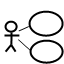
\includegraphics[scale=0.5]{use-case-diagram.png}} & #1 \tabularnewline
\hline
\raisebox{-0.8\height}{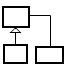
\includegraphics[scale=0.5]{class-diagram.png}} & #2 \tabularnewline
\hline
\raisebox{-0.8\height}{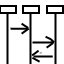
\includegraphics[scale=0.5]{sequence-diagram.png}} & #3 \tabularnewline
\hline
\raisebox{-0.8\height}{
\includegraphics[scale=0.5]{interrogation.png}} & #4
\end{tabular}\vfill\end{center}\end{minipage}};
\end{tikzpicture}\hspace{-1mm}}

\newcommand{\instruction}{\textit}

\newcommand{\newrow}{}

\newcommand{\challenge}{
\includegraphics[scale=0.05]{sun.jpg}}

\begin{document}


\umlpiccard
{Les activités de "Top Mobilier" sont la vente "multiproduits"(objets de décoration) et la vente de meubles; celle-ci se fait "à emporter"ou "en livraison"
}
{Un tabouret et une chaise sont des sortes de sièges qui ont respectivement 3 et 4 pieds.
}
{\emph{Choisir n'importe quelle autre question sur la carte}
}
{Alice insère sa carte dans le DAB qui lui demande son code, elle l'entre, le DAB lui demande combien elle veut retirer, Alice répond 50, elle reçoit l'argent, sa carte et un reçu.
}
\umlpiccard
{\emph{Relancer le dé}
}
{Une pièce contient des murs.
}
{Fred demande 20 euros à sa mère, qui le les lui donne après être allée les retirer au distributeur.
}
{\challenge Qui s'y frotte s'y pique.
}
\umlpiccard
{Sur cette machine à café, on peut insérer de l'argent, demander une boisson, ou obtenir un remboursement.
}
{La vie est une sorte de boite de chocolats.
}
{Qui vole un œuf vole un bœuf. 
}
{\emph{Relancer le dé}
}
\umlpiccard
{Dans une vente immobilière, il y a un vendeur et un acheteur.
}
{\challenge Tout chien qui aboie ne mord pas.
}
{Tomber 6 fois se relever 7
}
{Il y a 2 sortes de cowboys, ceux qui ont le revolver et ceux qui creusent
}

\newrow
\umlpiccard
{\challenge Avec le téléphone, on peut appeler ou être appelé.
}
{\challenge Les animaux sont soit des herbivores soit des carnivores soit des omnivores qui mangent donc soit des végétaux, d'autres animaux ou les deux.
}
{Aide toi, le ciel t'aidera
}
{Un père tend sa montre à son fils et lui demande l'heure qu'il est. Son fils lui répond : 9:00
}
\umlpiccard
{\emph{Choisir n'importe quelle autre question sur la carte}
}
{Le monde est composé de 2 catégories de personnes : les loosers et les tricheurs
}
{\challenge Papa : "va demander à ta mère pour avoir l'autorisation de sortir et avertis moi de sa décision"
}
{les rectangles et les triangles sont des polygones ; un polygone comporte au moins trois segments.
}
\umlpiccard
{Un usager se déplace grâce à un ascenseur ; l'exploitant configure l'ascenseur ; le réparateur effectue la maintenance
}
{\challenge La femme est l'avenir de l'homme.
}
{l'homme propose, la femme dispose
}
{\emph{Répondre à la question ? de cette carte} 
}
\umlpiccard
{Dans un distributeur de DVD géré par un franchisé on peut consulter les titres disponibles, emprunter ou rendre un DVD.
}
{\challenge \emph{Relancer le dé}
}
{\emph{Relancer le dé}
}
{\challenge \emph{Relancer le dé}
}

\newrow
\umlpiccard
{\emph{Choisir n'importe quelle autre question sur la carte}
}
{La vie est un long fleuve tranquille
}
{Le dessinateur tire une carte, dessine, et son équipe trouve la solution avant que le sablier soit vide
}
{Alice compose le 18, l'opérateur lui demande des informations, Alice les le lui donne, l'opérateur déclenche l'envoi des pompiers.
}
\umlpiccard
{\challenge Jésus crie, la caravane passe et les ciseaux aboient
}
{Une ressource est une image, une applet, ou un document html ; elle peut faire référence à d'autres ressources.
}
{Le prof dit : "va faire signer ton carnet de note par tes parents" et l'élève s'exécute.
}
{Plusieurs bâtiments peuvent avoir la même adresse.
}
\umlpiccard
{\emph{Relancer le dé}
}
{\challenge Le chat est un mammifère quadrupède sachant marcher et courir.
}
{\emph{Choisir n'importe quelle autre question sur la carte}
}
{\challenge l'homme propose, la femme dispose
}
\umlpiccard
{Les abonnés peuvent emprunter des cassettes VHS et des DVD; ils peuvent consulter le catalogue général.
}
{Les entrepôts servent à stocker des produits avec une quantité de produit dans chacun.
}
{L'appartement est nettoyé à chaque départ du locataire et une vérification de l'inventaire est effectuée.
}
{Le centre de documentation central (CDC) tient à jour le catalogue des ouvrages. Tous les mois, il le transmet aux CDL (locaux) par messagerie.
}

\newrow
\umlpiccard
{\challenge Une partie oppose deux joueurs, dont l'un a la main.
}
{\challenge Le monde est composé de 3 catégories de personnes : ceux qui savent compter et les autres.
}
{\challenge Tel est pris qui croyait prendre.
}
{Au jeu de boules, on peut lancer le cochonnet, tirer ou placer une boule, puis les ramasser.
}
\umlpiccard
{\emph{Répondre à la question ? de cette carte} 
}
{Les chats sont des félidés, les chiens sont des canidés, ces deux familles font partie des mammifères.
}
{Tu mets une ou des pièces dans le distributeur, et tu choisis ta boisson.
}
{\challenge Pour ta boisson, tu peux choisir des compléments tels que lait ou sucre.
}
\umlpiccard
{\emph{Relancer le dé}
}
{\challenge Les animaux se déplacent dans l'eau, dans l'air ou sur le sol; les phoques se déplacent dans l'eau ou sur le sol, les vautours en l'air ou sur le sol.
}
{En fin de semaine, les demandes sont regroupées dans des commandes passées auprès des fournisseurs.
}
{Le joueur a insulté l'arbitre; il a reçu un carton rouge et a été expulsé.
}
\umlpiccard
{Les ventes de meubles sont traitées par les vendeurs : prise de commande, modification, annulation.
}
{\challenge Mon nom est personne
}
{Le sourire que tu envoies revient vers toi (sagesse hindoue)
}
{\challenge être ou ne pas être, telle est la question.
}

\newrow
\umlpiccard
{\challenge Le matériel peut être affecté à une salle, ou être  indépendant (=mobile)
}
{Un arbre de Noël est décoré par des boules, des guirlandes, et des denrées périssables telles que fruits, bonbons, ...
}
{Au sein d'une entreprise un numéro interne de téléphone a quatre chiffres et ne commence pas par 0. Pour appeler l'extérieur, composer le 0, puis le numéro  à 10 chiffres.
}
{\challenge \emph{Choisir n'importe quelle autre question sur la carte}
}
\umlpiccard
{\challenge Aide toi, le ciel t'aidera 
}
{Les hommes et les femmes peuvent portent des vêtements tels que pantalon, veste; les femmes portent aussi des robes
}
{Et Dieu dit : "que la lumière soit" et la lumière fut
}
{\challenge Mr et Mme Ragetourne ont une fille : Sylvie
}
\umlpiccard
{Dans un débat public mené sur Internet, un animateur donne successivement la parole à des intervenants et peut prendre des questions dans le public.
}
{\challenge L'homme est loup pour l'homme
}
{Bob insère sa carte dans le lecteur, la porte s'ouvre, Bob entre dans le bâtiment, la porte se ferme
}
{Pour faire un cours, il faut, une salle, un prof et des élèves
}
\umlpiccard
{Un gestionnaire de vente à distance maintient un catalogue qu'on peut consulter pour éventuellement acheter en ligne et être livré.
}
{Les élèves ont une note dans chaque matière
}
{\challenge L'air est successivement comprimé par chacun des 3 pistons du compresseur avant d'être stocké dans un bloc tampon.
}
{\challenge Tous les chats savent miauler
}

\newrow
\umlpiccard
{\emph{Répondre à la question ? de cette carte} 
}
{\challenge Tous les oiseaux savent voler, sauf les autruches et les poules qui marchent et les pingouins qui nagent.
}
{Le dessinateur tire une carte, dessine, mais son équipe ne trouve pas la solution avant que le sablier soit vide
}
{Un menu comprend soit une entrés et un plat, soit un plat et un dessert
}
\umlpiccard
{Sur un DAB, on peut retirer du liquide, en déposer, encaisser des chèques et imprimer un RIB
}
{Il existe 2 sortes de trucs, les trucs simples et les trucs composés. Les trucs composés sont composés de trucs.
}
{Le 5 février un client achète un meuble en magasin. Le vendeur saisit la commande et téléphone au Centre d'appels pour convenir d'une livraison le 15 février.
}
{\emph{Choisir n'importe quelle autre question sur la carte}
}
\umlpiccard
{\emph{Relancer le dé}
}
{Dans une voiture, il y a obligatoirement un feu arrière de brouillard et exceptionnellement un feu avant de brouillard.
}
{\challenge L'arbre à cames transmet l'énergie du moteur aux roues
}
{\challenge Tant va la cruche à l'eau qu'à la fin elle se casse
}
\umlpiccard
{\challenge Dans UML Pictionnary il y a un dessinateur par équipe, les devins et les spectateurs.
}
{\challenge Dans une voiture, les clignotants, l'alarme sonore, les warnings et les essuies-glace sont des dispositifs tout ou rien cadencés.
}
{\challenge Un verre ça va, 3 verres, bonjour les dégâts
}
{Le bon, la brute et le truand sont des cow-boys.
}

\newrow
\umlpiccard
{\challenge Dans un restaurant on trouve des clients, des serveurs, un maitre d'hôtel, des cuisiniers et un sommelier.
}
{\challenge Les ennemis de mes ennemis sont mes amis
}
{Alice compose un numéro, le téléphone de Bob sonne, Bob décroche, ils parlent, Bob raccroche.
}
{\emph{Choisir n'importe quelle autre question sur la carte}
}
\umlpiccard
{\challenge Lors d'une conférence, après que l'orateur a fini de parler, le président de séance accorde la parole à un ou plusieurs auditeurs pour poser des questions auxquels l'orateur répond.
}
{L'argent est le nerf de la guerre 
}
{\challenge métro, boulot, dodo
}
{\challenge La religion est l'opium du peuple
}
\umlpiccard
{\emph{Relancer le dé}
}
{Au contraire des bicyclettes, les voitures, les bus et les camions sont des sortes de véhicules ayant un moteur diesel ou essence.
}
{Alice insère sa carte dans le DAB qui lui demande son code, elle l'entre, le DAB lui demande combien elle veut retirer, Alice répond 50, elle reçoit l'argent, sa carte et un reçu.
}
{\emph{Répondre à la question ? de cette carte} 
}
\umlpiccard
{\emph{Relancer le dé}
}
{Un répertoire contient des fichiers ou d'autres répertoires connus par leur nom.
}
{Bob insère sa carte dans la pompe automatique, compose son code, prend de l'essence et obtient un reçu.
}
{Dans une liste de diffusion modérée, il y a un modérateur qui contrôle le contenu des messages envoyés sur la liste.
}

\newrow
\umlpiccard
{\emph{Répondre à la question ? de cette carte} 
}
{\challenge Les animaux se déplacent dans l'eau, dans l'air ou sur le sol; les phoques se déplacent dans l'eau ou sur le sol, les vautours en l'air ou sur le sol.
}
{\challenge La rumeur a circulé parmi les habitants avant que le maire l'apprenne.
}
{Les rectangles et les triangles sont des polygones; un polygone comporte au moins trois segments, comme bords.
}
\umlpiccard
{\emph{Choisir n'importe quelle autre question sur la carte}
}
{\challenge Une personne peut être embauchée plusieurs fois chez le même employeur et peut avoir exercé plusieurs fonctions chez le même employeur ou la même fonction chez des employeurs différents.
}
{\emph{Choisir n'importe quelle autre question sur la carte}
}
{Le centre de documentation central(CDC) tient à jour le catalogue des ouvrages. Tous les mois, il le transmet aux CDL (locaux) par messagerie.
}
\umlpiccard
{L'appartement est nettoyé à chaque départ du locataire et une vérification de l'inventaire est effectuée.
}
{\challenge Un homme et une femme peuvent se marier, deux personnes peuvent se pacser.
}
{Chaque personne qui reçoit ce "message de l'amitié" doit le transmettre à 2 autres et il sera heureux, sinon des malheurs lui arriveront 
}
{Une pièce contient des murs.
}
\umlpiccard
{Les ventes de meubles sont traitées par les vendeurs : prise de commande, modification, annulation.
}
{Une ressource est une image, une applet, ou un document html ; elle peut faire référence à d'autres ressources.
}
{Si l'appartement est en bon état, le contrat entre le propriétaire et la société peut être renouvelé.
}
{L'appartement est nettoyé à chaque départ du locataire et une vérification de l'inventaire est effectuée.
}

\newrow
\umlpiccard
{\challenge 1ère loi de la robotique : Un robot ne peut porter atteinte à un être humain ni, restant passif, laisser cet être humain exposé au danger.
}
{Il y a 10 sortes de personnes, ceux qui connaissent le binaire et les autres.
}
{\challenge Le sourire que tu envoies revient vers toi (sagesse hindoue)
}
{Tirez une autre carte}
\umlpiccard
{Tirez une autre carte}
{Tirez une autre carte}
{Au jeu de boules : "tu tires sa boule et je place derrière"
}
{Le joueur a insulté l'arbitre; il a reçu un carton rouge et a été expulsé.
}
\umlpiccard
{Tirez une autre carte}
{Tirez une autre carte}
{Tirez une autre carte}
{Tirez une autre carte}

%\umlpiccard
%{Les activités de "Top Mobilier"
%sont la vente "multiproduits" (objets de décoration) et la vente de
%meubles; celle-ci se fait "à
%emporter"ou "en livraison"}
%{Un tabouret et une chaise sont
%des sortes de sièges qui ont
%respectivement 3 et 4 pieds.}
%{\instruction{Choisir n'importe quelle autre
%question sur la carte}}
%{Avec le téléphone, on peut appeler
%ou être appelé.}
%%
%%
%%
%\umlpiccard
%{\instruction{Relancer le dé}}
%{Une pièce contient des murs.}{Alice insère sa carte dans le
%DAB qui lui demande son
%code, elle l'entre, le DAB lui
%damande combien elle veut
%retirer, Alice répond 50, elle
%recoit l'argent, sa carte et
%un recu.}
%{\instruction{Relancer le dé}}
%%
%%
%\umlpiccard{Sur cette machine à café, on
%peut insérer de l'argent, demander
%une boisson, ou obtenir
%un remboursement.}
%{La vie est une sorte de boite
%de chocolats.}
%{Fred demande 20 euros à sa
%mère, qui le les lui donne
%après être allée les retirer au
%distributeur.}
%{Jésus crie, la caravane passe
%et les ciseaux aboient.}
\end{document}


